\documentclass[aspectratio=169,xcolor=dvipsnames]{beamer}
\usetheme{SimplePlus}
\usepackage{hyperref}
\usepackage{graphicx}
\usepackage{booktabs} 
\usepackage{tikz}
\usepackage {mathtools}
\usepackage[utf8]{inputenc}
\usepackage[french]{babel}
\usepackage{listings}
\usepackage{array}
\usepackage[ruled,vlined]{algorithm2e}
\usepackage{algpseudocode}
\usepackage{caption}
\usepackage{subcaption}
\usepackage{float}
\usepackage[T1]{fontenc}

\title{Soutenance - Conception Logicielle Analyseur LVDEH}
\author{Baptiste Borie, Benjamin Boutrois, Nazar Ulan, Daphné Larrivain}
\date{Avril 2023}

\begin{document}

\maketitle
\begin{frame}
\tableofcontents
\end{frame}

\section{Introduction}
\begin{frame}{Introduction}
\begin{center}
    \huge Livre dont vous êtes le Héro
\end{center}
 
 4 parties :
 \begin{center}
    \begin{itemize}
        \item Lecteur de fichiers et structure de donnée
        \item Graphique 
        \item Métrique
        \item Interface graphique
    \end{itemize}
    \end{center}
\end{frame}
\section{Stockage des données et convertisseurs}
\begin{frame}{Stockage des données et convertisseurs}
    \begin{center}
    \begin{itemize}
        \item Stockage du livre
        \item Convertisseur de fichiers
    \end{itemize}
    \end{center}
\end{frame}
\subsection{Stockage du livre}
\begin{frame}{Stockage du livre}
    \begin{center}
         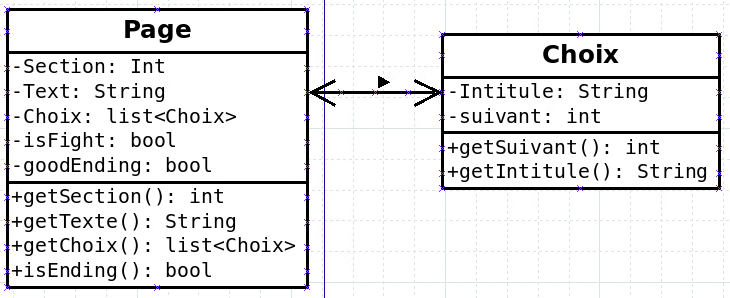
\includegraphics[width=0.8\textwidth]{diagramme_page.png}{\small\textsl{\\Diagramme des objets Page et Choix}}
    \end{center}
\end{frame}
\subsection{Convertisseurs JSON et TXT}
\begin{frame}{Convertisseurs JSON et TXT}
                \begin{center}
            \begin{minipage}{.33\textwidth}
    \centering
        \vspace{1cm}
        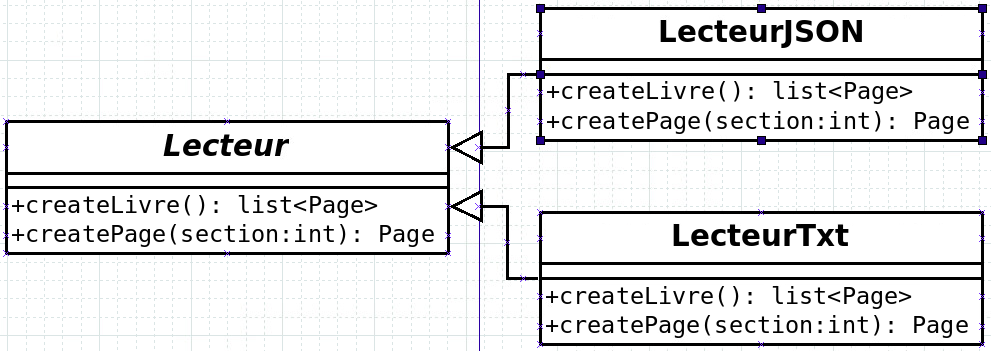
\includegraphics[width=1.2\textwidth]{diagramme_lecteurs.png}{\small\textsl{\\Diagramme des lecteurs}}
        \end{minipage}
        \begin{minipage}{.66\textwidth}
        \centering
        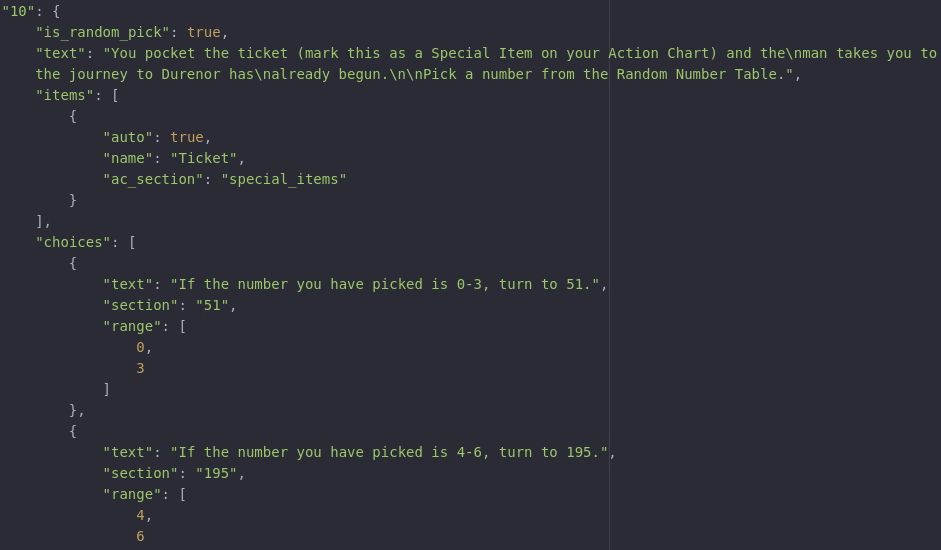
\includegraphics[width=0.6\textwidth]{livre_json.png}
        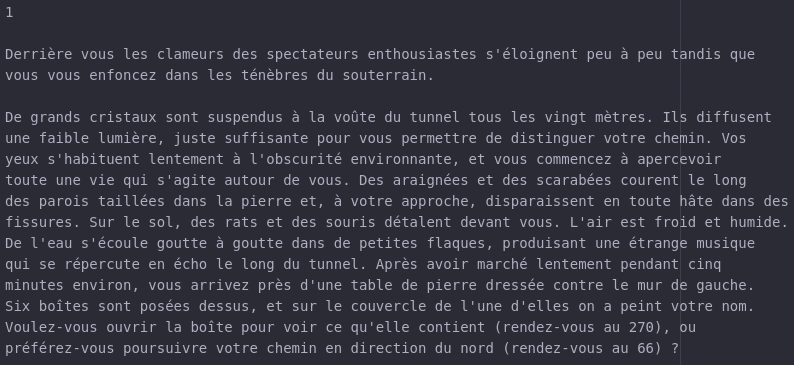
\includegraphics[width=0.6\textwidth]{livre_txt.png}
    \end{minipage}
    \end{center}
\end{frame}

\section{Les calculs métrique}
\begin{frame}{Les calculs métrique}
    \begin{center}
    \begin{itemize}
        \item Algorithmes utilisés
        \item Agrégation de données
        \item Résultats obtenus
    \end{itemize}
    \end{center}
\end{frame}
\subsection{Algorithmes utilisés}
\begin{frame}{Algorithmes utilisés dans la partie Métrique}
Dans le processus d'écriture du code de calcul de la métrique, 3 algorithmes principaux ont été utilisés.:
\begin{itemize}
\item 'Agrégation de données'
qui nous a aidé à calculer des statistiques générales des livres
\item 'Algorithme de parcours en largeur' grâce auquel nous avons calculés les chemins le plus courts
\item 'Algorithme de parcours en profondeur' grâce auquel nous avons calculés les chemins le plus longs
\end{itemize}
\end{frame}
\setbeamercovered{transparent}

\subsection{Agrégation de données}
\begin{frame}{Agrégation de données}
\begin{figure}
\centering
  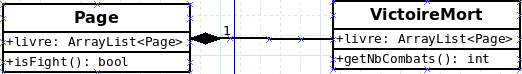
\includegraphics[width=65mm,scale=0.5]{agregation.png}
  \caption{Exemple d'agrégation de données}
  \label{fig:boat1}
\end{figure}
\end{frame}

\begin{frame}{Algorithme de parcours en largeur(BFS) et en longueur(DFS)}
\begin{figure}
\centering
  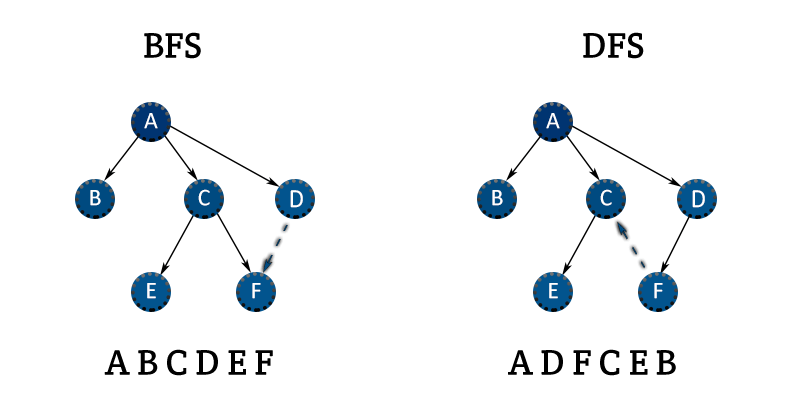
\includegraphics[width=100mm,scale=0.5]{BFS-DFS.png}
  \caption{Exemples des algorithmes}
\end{figure}

\end{frame}

\subsection{Résultats obtenus}
\begin{frame}{Résultats obtenus}
\begin{figure}
\centering
  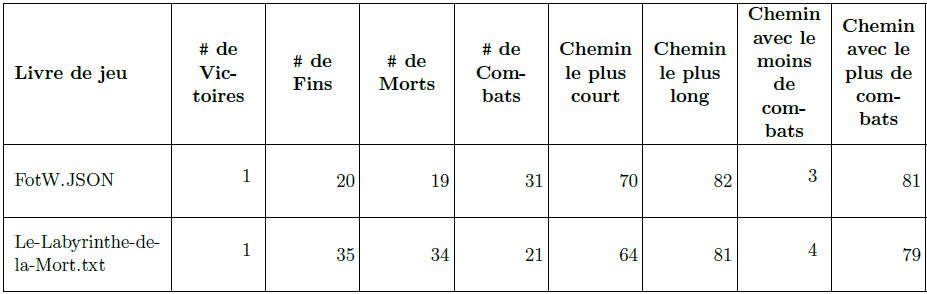
\includegraphics[width=100mm,scale=0.5]{stats.png}
  \caption{Statistiques des livres}
\end{figure}
\end{frame}

\begin{frame}{Défauts dans l'affichage des métriques}
\begin{figure}
\centering
  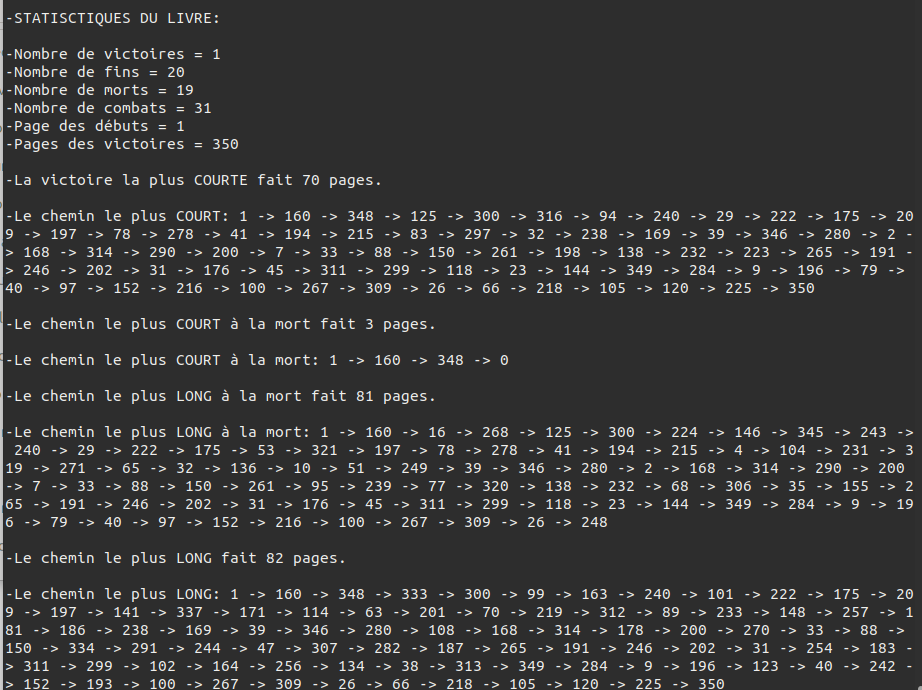
\includegraphics[width=100mm,scale=0.5]{livreJSON.png}
  \caption{Livre JSON}
\end{figure}
\end{frame}

\begin{frame}{Défauts dans l'affichage des métriques}
\begin{figure}
\centering
    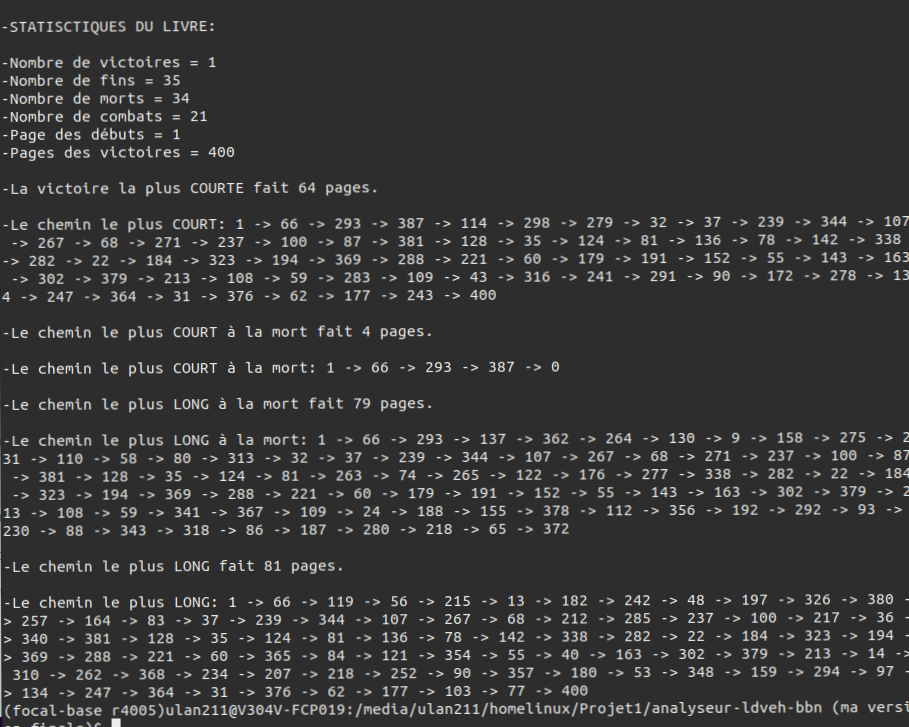
\includegraphics[width=95mm,scale=0.5]{livreTXT.png}
  \caption{Livre TXT}
\end{figure}
\end{frame}

\section{Graphe}
\begin{frame}{Graphe}
    \begin{center}
    \begin{itemize}
        \item Kamada Kawai
        \item Interface graphique
        \item Exemple d'application
    \end{itemize}
    \end{center}
\end{frame}
\subsection{Kamada Kawai}
    \begin{frame}{Principe}
        \begin{algorithm}[H]
        \caption{Pseudo-code de l'algorithme de Kamada-Kawai}\label{alg:cap}
        \SetKwInOut{Input}{Entrée}
        \SetKwInOut{Output}{Sortie}
        \SetKwInOut{Compute}{Compute}
        \SetKwInOut{Init}{Initialize}
        
        \Compute{$d_{ij}$ for $1 \leq i \ne j \leq n$}
        \Compute{$l_{ij}$ for $1 \leq i \ne j \leq n$}
        \Compute{$k_{ij}$ for $1 \leq i \ne j \leq n$}
        \Init{$p_1, p_2, ..., p_n$}
        
        \While{$max_i \Delta_i > \mu $}{
        let $p_m$ be the particule satisfying $\Delta_m = max_i \Delta_i$;\\
        \While{$\Delta_m > \mu $}{
        compute $\delta x, \delta y$;\\
        $x_m := x_m + \delta x$;\\
        $y_m := y_m + \delta y$;
        }
        }
        \end{algorithm}
    \end{frame}
    
\subsection{Interface graphique}
    \begin{frame}{Interface graphique}
        \begin{figure}
        \centering
            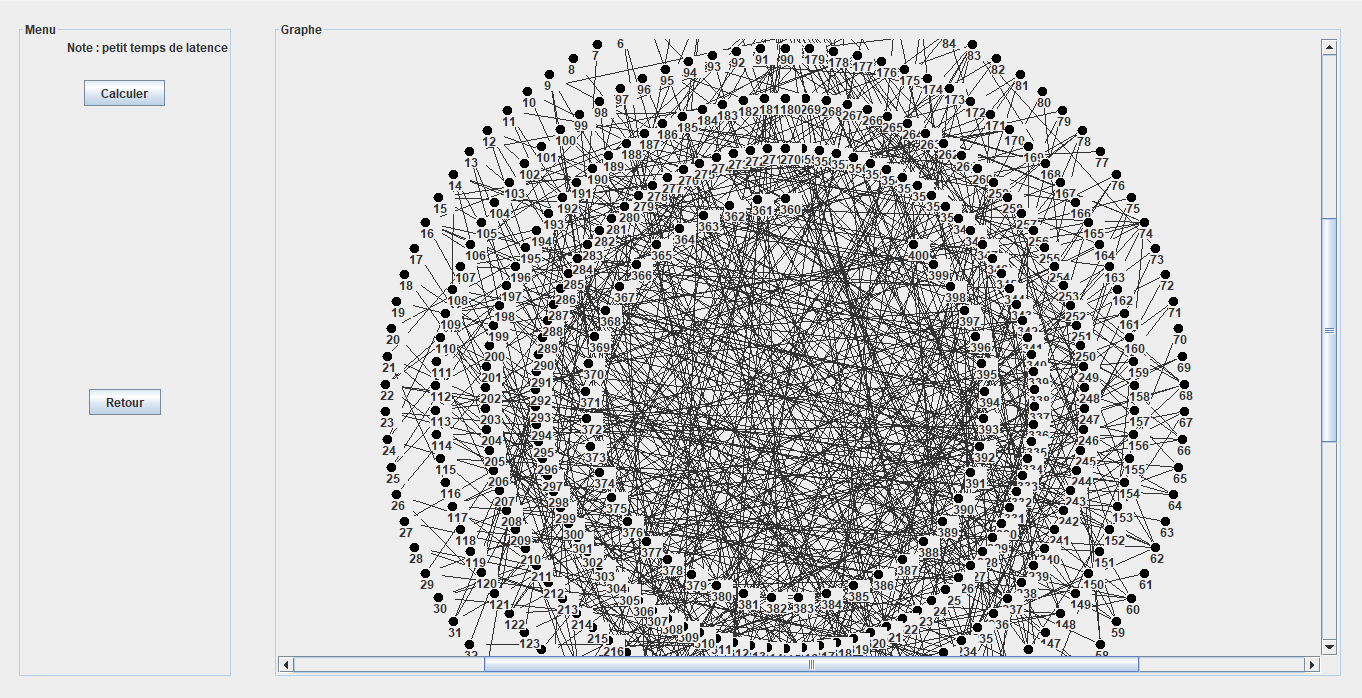
\includegraphics[width=0.9\textwidth]{interface.png}
            \caption{Avec initialisation sur 400 noeuds}
            \label{fig:interface}
        \end{figure}	
    \end{frame}

\subsection{Exemple d'application}
    \begin{frame}{Exemple d'application}
        \begin{figure}
        \centering
            \begin{subfigure}[b]{0.4\textwidth}
                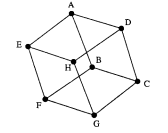
\includegraphics[width=\textwidth]{cube_des.png}
                \caption{Résultat attendu}
                \label{fig:cube}
            \end{subfigure}
            \begin{subfigure}[b]{0.4\textwidth}
                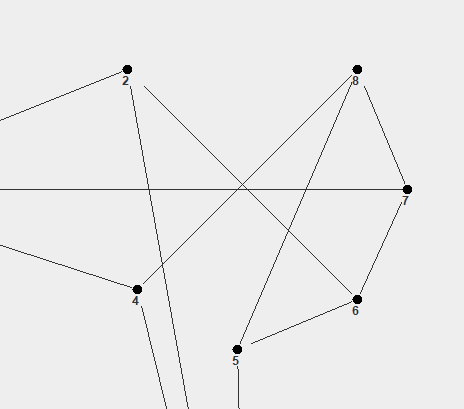
\includegraphics[width=\textwidth]{cube_err.png}
                \caption{Résultat obtenu}
                \label{fig:cube_err}
            \end{subfigure}
        \label{fig:images}
        \end{figure}
    \end{frame}

\section{L'interface graphique}
\begin{frame}{L'interface graphique}
    \begin{center}
    \begin{itemize}
        \item Charte Graphique
        \item Interface du jeu
    \end{itemize}
    \end{center}
\end{frame}

\subsection{Charte Graphique}
\begin{frame}{Charte Graphique}
        \begin{center}
            \begin{minipage}{.49\textwidth}
    \centering
        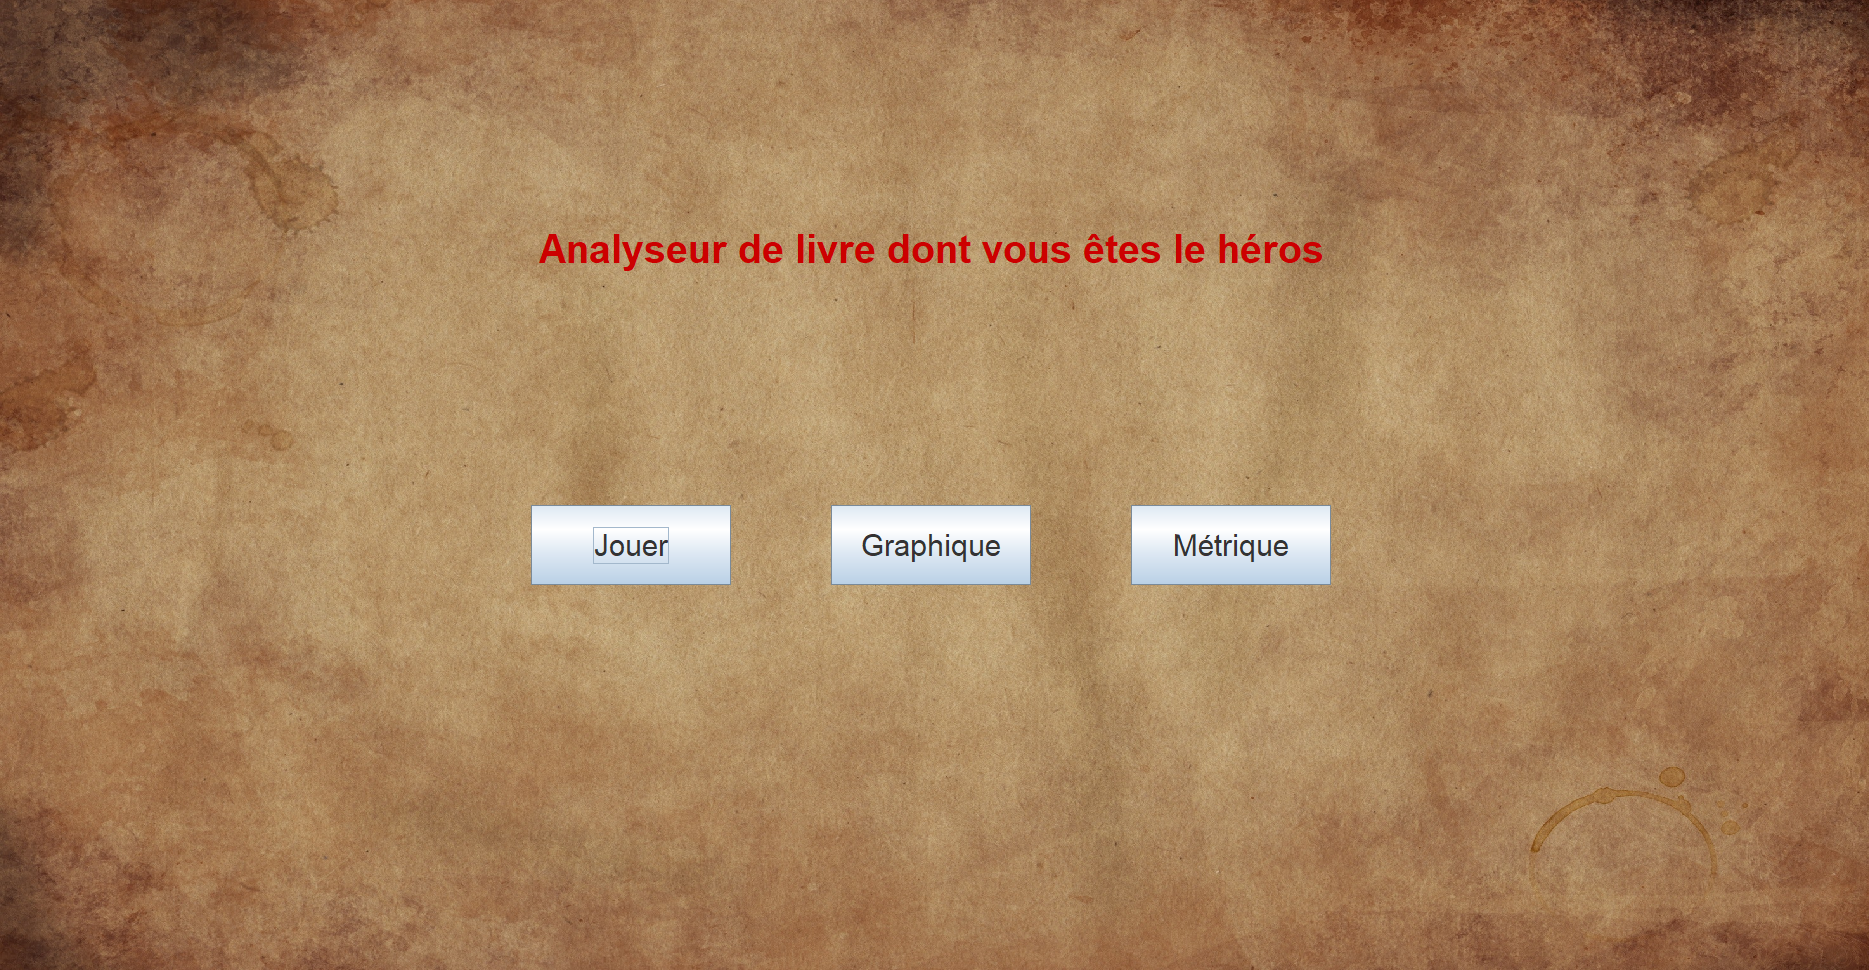
\includegraphics[width=\textwidth]{imgMenu.png}{\small\textsl{\\Ecran de menu }}
        \end{minipage}
        \begin{minipage}{.49\textwidth}
        \centering
        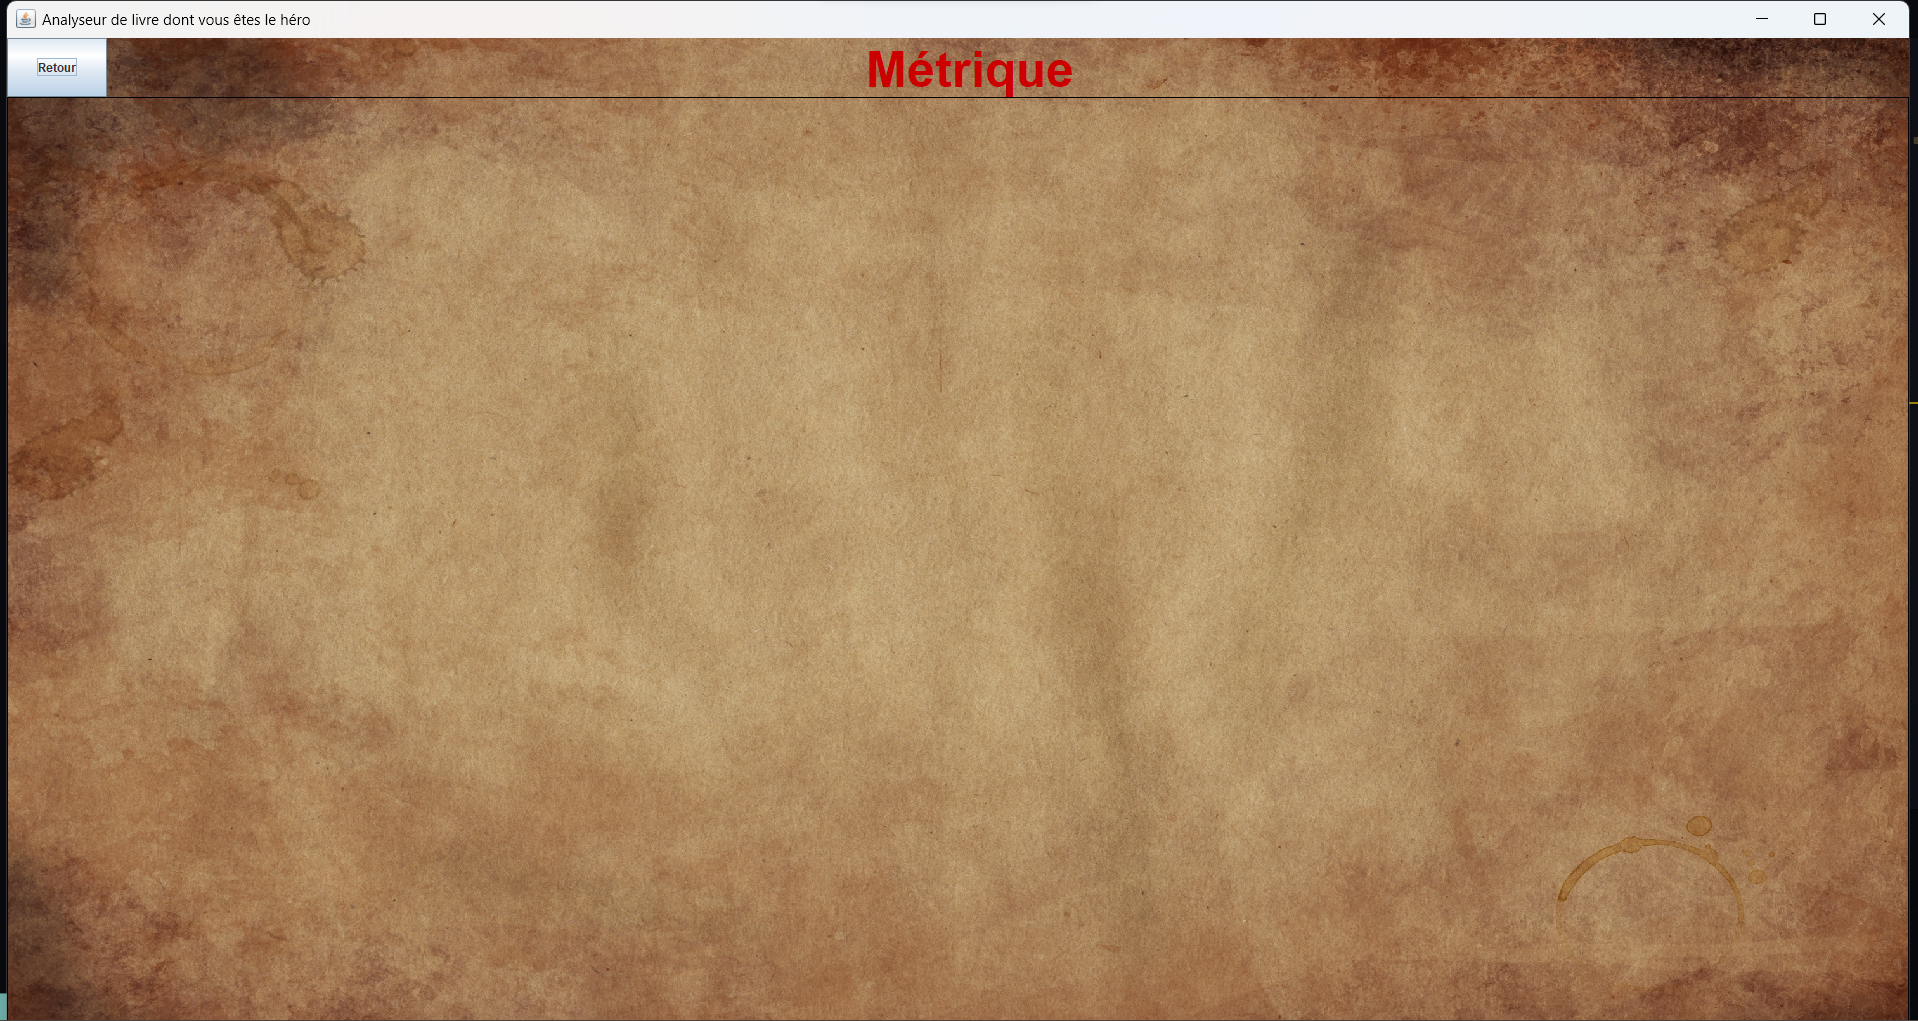
\includegraphics[width=\textwidth]{structureGUI.png}{\small\textsl{\\Aspect d'une page sans contenu.}}
    \end{minipage}
    \end{center}
\end{frame}
\subsection{Interface de jeu}
\begin{frame}{Interface de jeu}
       \centering
    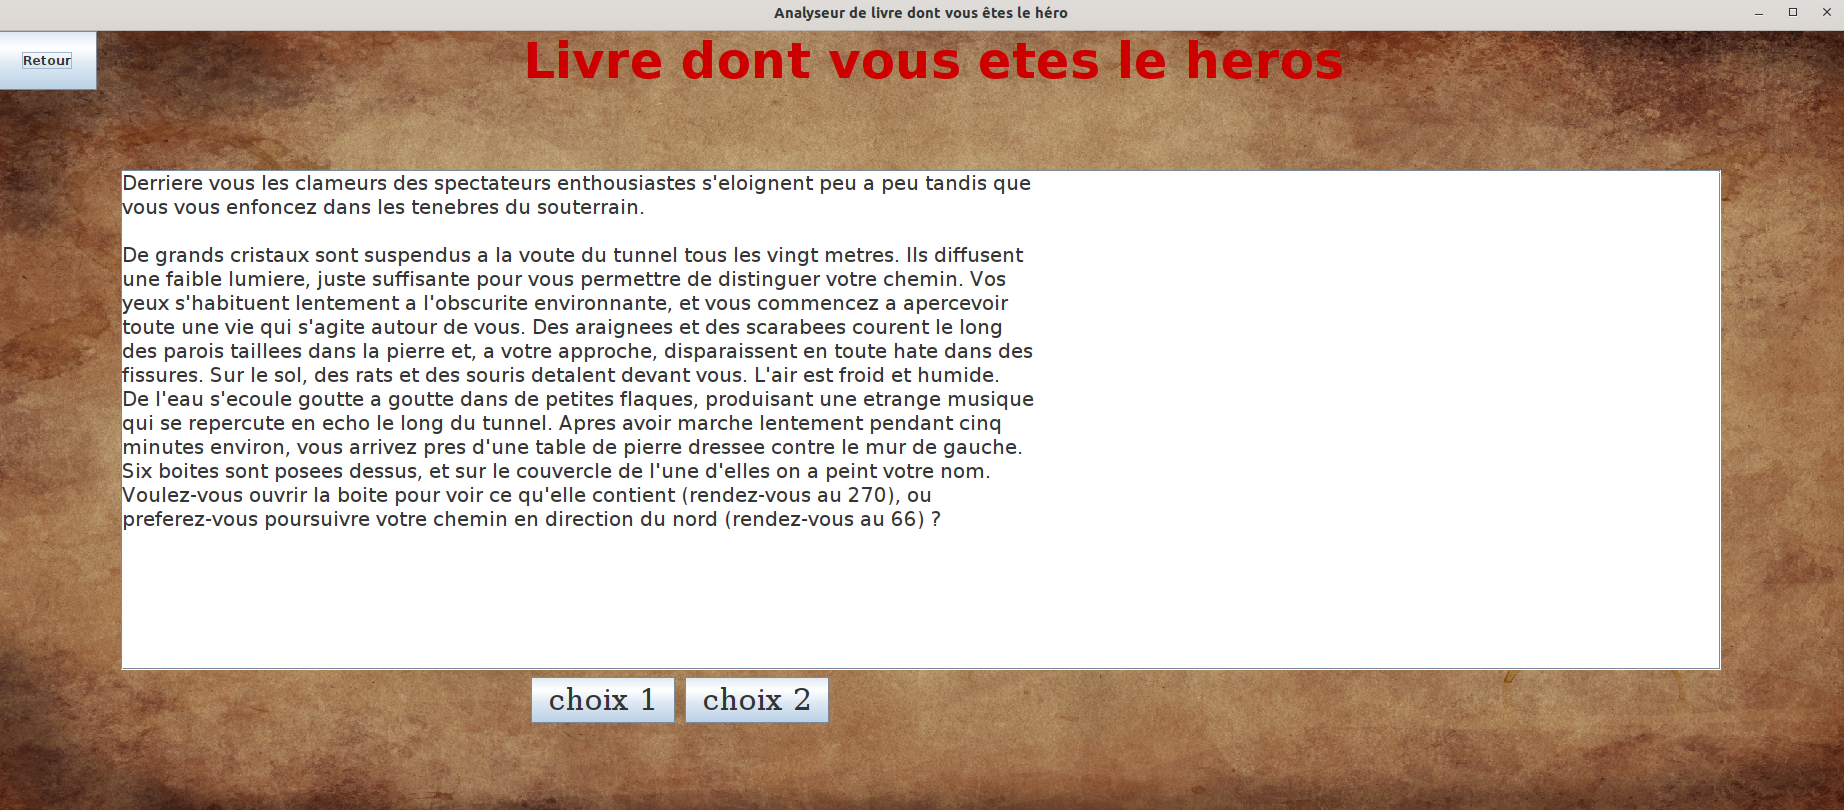
\includegraphics[width=\textwidth]{imageJeu.png}{\small\textsl{\\Rendu en jeu}}
\end{frame}
\section{Conclusion}
\begin{frame}{Conclusion}
    \begin{center}
        \huge Conclusion  
    \end{center}
       {\small\textsl{Projet réalisé par Baptiste Borie, Benjamin Boutrois, Nazar Ulan, Daphné Larrivain }}
\end{frame}




\end{document}
